\documentclass[titlepage]{article}
\usepackage[top=2cm,left=2.5cm,right=2.5cm,bottom=2cm]{geometry}
\usepackage{graphicx}
\graphicspath{ {images/} }


\title{{\Huge Multiplayer Snake}\\\vspace{3mm}{\large Software Engineering 1 \& Intro to Java}}
\date{\today}
\author{{\normalsize by}\\{\large Ian Laird \& Andrew Walker}\\ \\ {\normalsize prepared for}\\Dr. Tomas Cerny}

\begin{document}
	\maketitle
	\section{Outline}
	This game implements a 2 player version of the popular game Snake. Communication between the host and client is done using TCP. Players can pick up power ups and kill the other player to increase their score. The player scores are saved in an XML file. Graphics are done using JavaFX for game setup and with Swing for the Game itself. The goal of the Game is to end with a higher score than the other player.

	\section{Vision Statement}
	The next step in this game will be making it so that more than 2 players can play at the same time. A further iteration of the software will have a dedicated Snake server that can run multiple games with more than 2 players concurrently.
	
	\section{Gantt}
	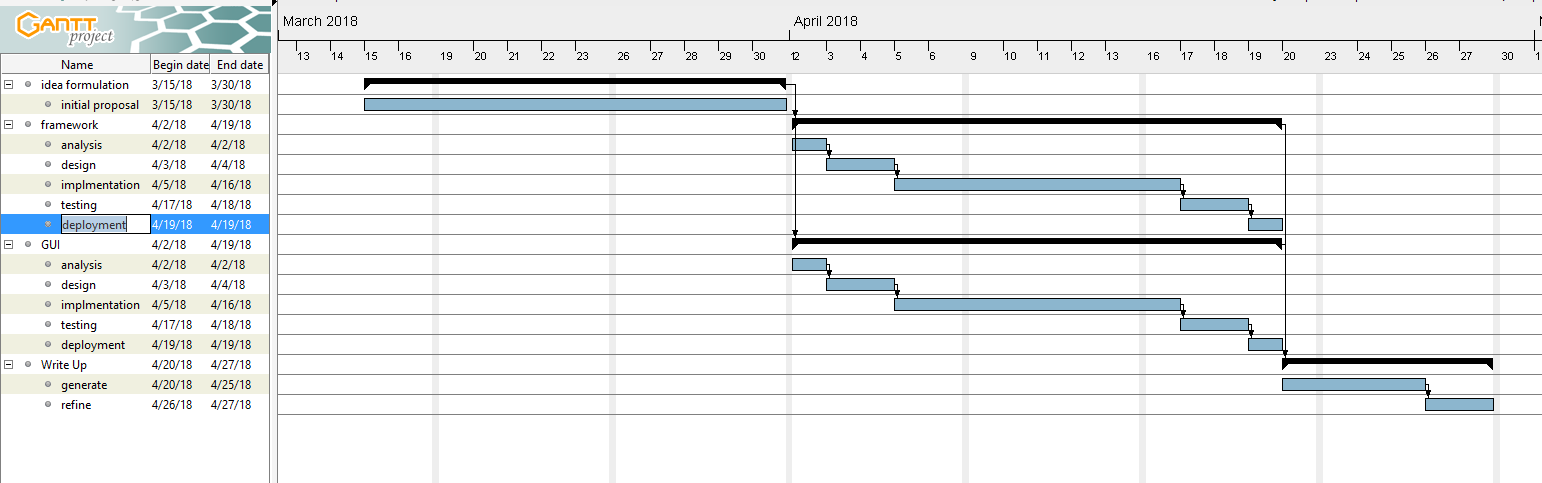
\includegraphics[scale=.50]{gantt2}
	
	\section{Requirements}
	\begin{enumerate}
		\item Game should run on any machine that supports Java.
		\item Game should play smoothly.
		\item Users should be able to view game score history.
		\item Game should have a GUI.
		\item Game should have a scoring system.
		\item Snakes should be able to increase in length.
		\item Users should be able to win/lose.
		\item Users should be able to play on separate computers over the internet.
		\item Users should be able to play again without restarting game.
	\end{enumerate}
	
	\section{Business Rules}
	
	\begin{enumerate}
		\item Client must know the ip address of the server.
		\item Each game must have two players.
		\item High scores are remembered.
	\end{enumerate}

	\section{All Roles}
	
	\begin{enumerate}
		\item Primary (Local) User - The user acting as the host for the game
		\item Secondary User - The user joining the hosted game
	\end{enumerate}
	
	\section{Use Cases}
	\subsection{Use Case 1}
	\itemsep0em 

			\textbf{\makebox[4 cm]{Name:\hfill}} UC1 -- Initialize Game\\
			\textbf{\makebox[4 cm]{Primary Actor:\hfill}} Local user\\
			\textbf{\makebox[4 cm]{Secondary Actor:\hfill}} Secondary user\\
			\textbf{\makebox[4 cm]{Trigger:\hfill}} Game is created\\
			\textbf{command.SnakeRunner Success Scenario}
				\begin{enumerate}
					\itemsep0em 
					\item[1] Primary and secondary users both want to play the game.
					\item[2] Network connection is established to secondary player.
					\item[3] Snakes and Tokens are generated with random locations.
					\item[4] Screen is created.
					\item[5] Game is now ready to be played.
				\end{enumerate}
			\textbf{Alternate Scenarios}
			\begin{enumerate}
									\itemsep0em 
				\item[1a]There is no secondary player to play with the primary player.
				\begin{enumerate}
										\itemsep0em 
					\item[1]System will wait until another player connects or user closes the application.
				\end{enumerate}
				\item[2a]network connection fails to establish.
				\begin{enumerate}
										\itemsep0em 
					\item[1]System will inform the user and then terminate.
				\end{enumerate}
				\item[3a]There is a collision where random locations are identical or very close to each other.
				\begin{enumerate}
										\itemsep0em 
					\item[1]Snake and Token Locations will be recalculated.
					\item[2]This process will be repeated until all positions are distinct and valid.
				\end{enumerate}
			\end{enumerate}
		
	\subsection{Use Case 2}
	\itemsep0em 
	
	\textbf{\makebox[4 cm]{Name:\hfill}} UC2 -- Play Game\\
	\textbf{\makebox[4 cm]{Primary Actor:\hfill}} Local user\\
	\textbf{\makebox[4 cm]{Secondary Actor:\hfill}} Secondary user\\
	\textbf{\makebox[4 cm]{Pre-condition:\hfill}} Game is created\\
	\textbf{command.SnakeRunner Success Scenario}
	\begin{enumerate}
		\itemsep0em 
		\item[1] Primary user makes and sends move.
		\item[2] Primary user receives secondary users move.
		\item[3] Each snake is replotted with the new position as the head.
	\end{enumerate}
	\textbf{Alternate Scenarios}
	\begin{enumerate}
		\itemsep0em 
		\item[a]Connection to other player is lost.
		\begin{enumerate}
			\itemsep0em 
			\item[1]System will notify player and terminate.
		\end{enumerate}
		\item[3a]Player is dead after move.
		\begin{enumerate}
			\itemsep0em 
			\item[1]Defeat screen is displayed.
			\item[2]Both players choose to play again and play resumes.
		\end{enumerate}
		\item[3b]Secondary player is dead after move.
		\begin{enumerate}
			\itemsep0em 
			\item[1]Victory screen is displayed.
			\item[2]Both players may choose to play again.
		\end{enumerate}
				\item[3ab.2a]Player chooses to not play again.
				\begin{enumerate}
					\itemsep0em 
					\item[1]High scores are updated.
					\item[2]Game terminates.
				\end{enumerate}
				\item[3ab.2b]Player 2 chooses to not play again.
				\begin{enumerate}
					\itemsep0em 
					\item[1]High scores are updated.
					\item[2]Game terminates.
				\end{enumerate}
	\end{enumerate}
		
	\subsection{Use Case 3}
	\itemsep0em 
	
	\textbf{\makebox[4 cm]{Name:\hfill}} UC3 -- Play Again\\
	\textbf{\makebox[4 cm]{Primary Actor:\hfill}} Local user\\
	\textbf{\makebox[4 cm]{Secondary Actor:\hfill}} Secondary user\\
	\textbf{\makebox[4 cm]{Pre-condition:\hfill}} Game over\\
	\textbf{\makebox[4 cm]{Post-condition:\hfill}} Game is not over\\
	\textbf{command.SnakeRunner Success Scenario}
	\begin{enumerate}
		\itemsep0em 
		\item[1] Snakes and Tokens are generated with random locations.
		\item[2] Screen is redrawn.
	\end{enumerate}
	\textbf{Alternate Scenarios}
	\begin{enumerate}
		\itemsep0em 
		\item[a]Connection to other player is lost.
		\begin{enumerate}
			\itemsep0em 
			\item[1]System will notify player and terminate.
		\end{enumerate}
	\item[1.a]Tokens and Snakes do not have independent positions.
			\begin{enumerate}
		\itemsep0em 
		\item[1]System will recalculate positions.
		\item[2]This will be repeated until all positions are independent of each other.
	\end{enumerate}
		
	\end{enumerate}
	
	\section{Use Case Diagram}
	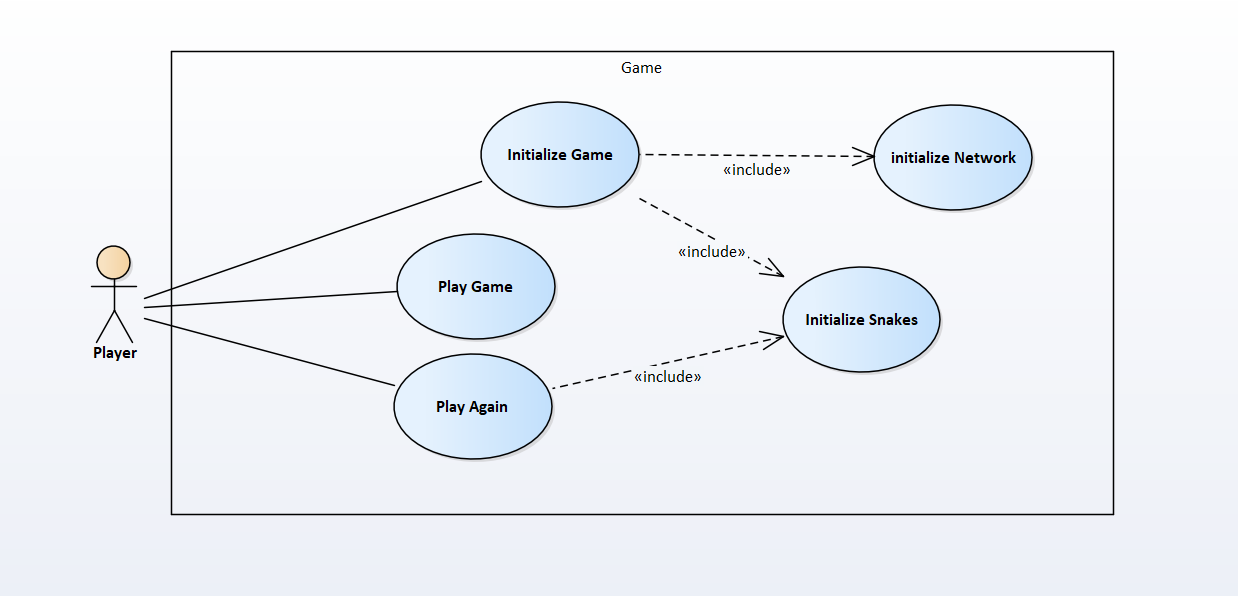
\includegraphics[scale=.75]{UCD}
	
	\section{System Sequence Diagram}
	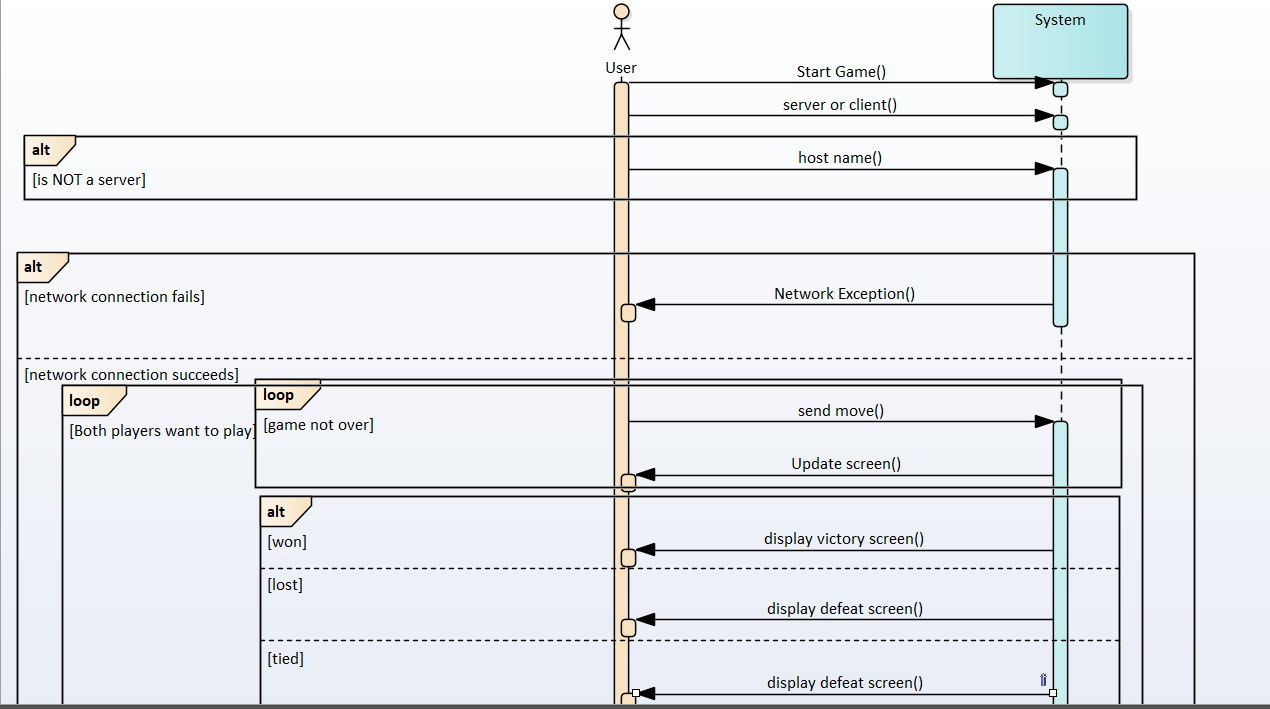
\includegraphics[scale=.75]{SSD}
	
	\section{System Operations}
	\begin{enumerate}
		\item $initGame()$
		\item $serverOrClient(boolean~mode)$
		\item $sendMove(Direction~move)$
	\end{enumerate}
	
	\section{Domain Model}
		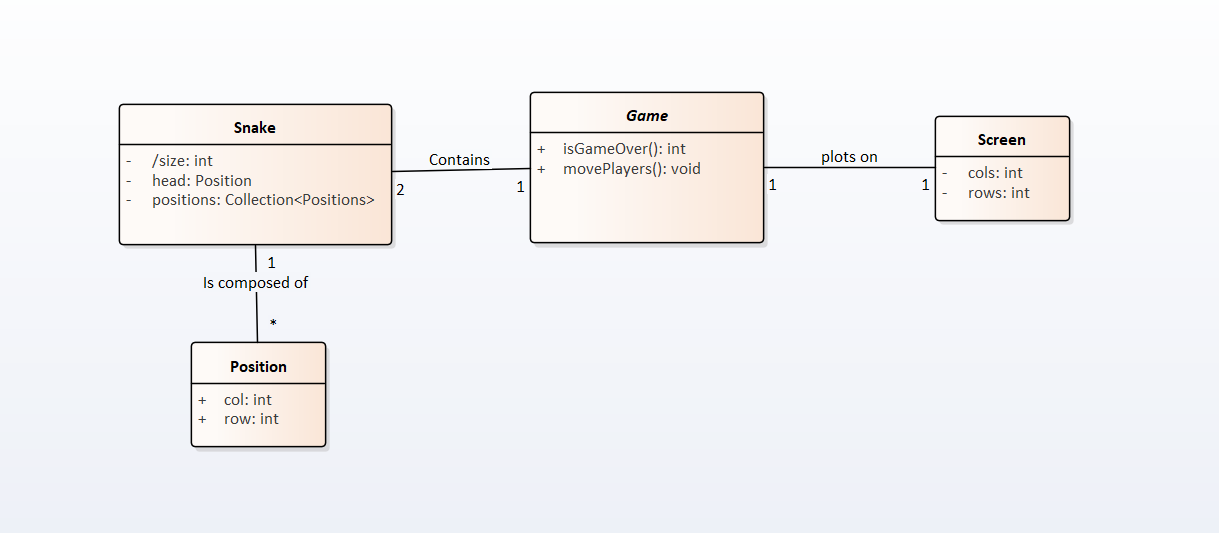
\includegraphics[scale=.75]{DM}
	
	\section{Operational Contracts}
	\subsection{Contract 1}
	\itemsep0em 
	
	\textbf{\makebox[4 cm]{Operation:\hfill}} initGame\\
	\textbf{\makebox[4 cm]{Cross References:\hfill}} UC1\\
	\textbf{\makebox[4 cm]{Pre-conditions:\hfill}} No instance of a Game exists\\
		\textbf{\makebox[4 cm]{Post-conditions:\hfill}} 
				\begin{itemize} 
				\item A Game is initialized.
				\end{itemize}
		
	\subsection{Contract 2}
	\itemsep0em 
	
	\textbf{\makebox[4 cm]{Operation:\hfill}} serverOrClient(boolean status)\\
	\textbf{\makebox[4 cm]{Cross References:\hfill}} UC1\\
	\textbf{\makebox[4 cm]{Pre-conditions:\hfill}} Game network has not been initialized previously.\\
	\textbf{\makebox[4 cm]{Post-conditions:\hfill}}
		\begin{itemize} 
			\item A socket has been initialized and connected to.
			\item If client, a connection will be made to server.
			\item If server, a client will be accepted.
		\end{itemize}
	
	\subsection{Contract 3}
	\itemsep0em 
	
	\textbf{\makebox[4 cm]{Operation:\hfill}} sendMove(Direction move)\\
	\textbf{\makebox[4 cm]{Cross References:\hfill}} UC2 and UC3\\
	\textbf{\makebox[4 cm]{Pre-conditions:\hfill}} Game has been initialized, and both players are still alive.\\
	\textbf{\makebox[4 cm]{Post-conditions:\hfill} }
	\begin{itemize} 
		\item Player one and player 2 are moved to new cells.
		\item If player does not make move, their last move will be repeated.
		\item If the received moves kill a player, that player will die. The other player will receive points.
	\end{itemize}
	
	
	
	\section{Sequence Diagrams}
	\subsection{Sequence Diagram 1 : Initialize Game}
	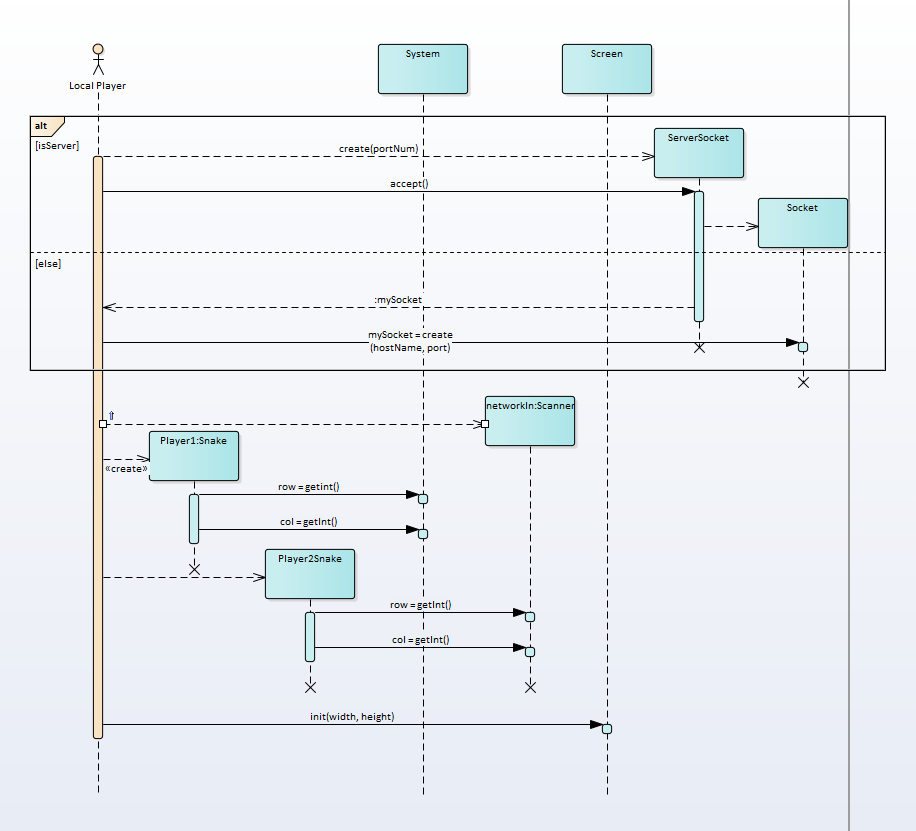
\includegraphics[scale=.75]{Sequence1}
	
	\subsection{Sequence Diagram 2 : Play Game}
	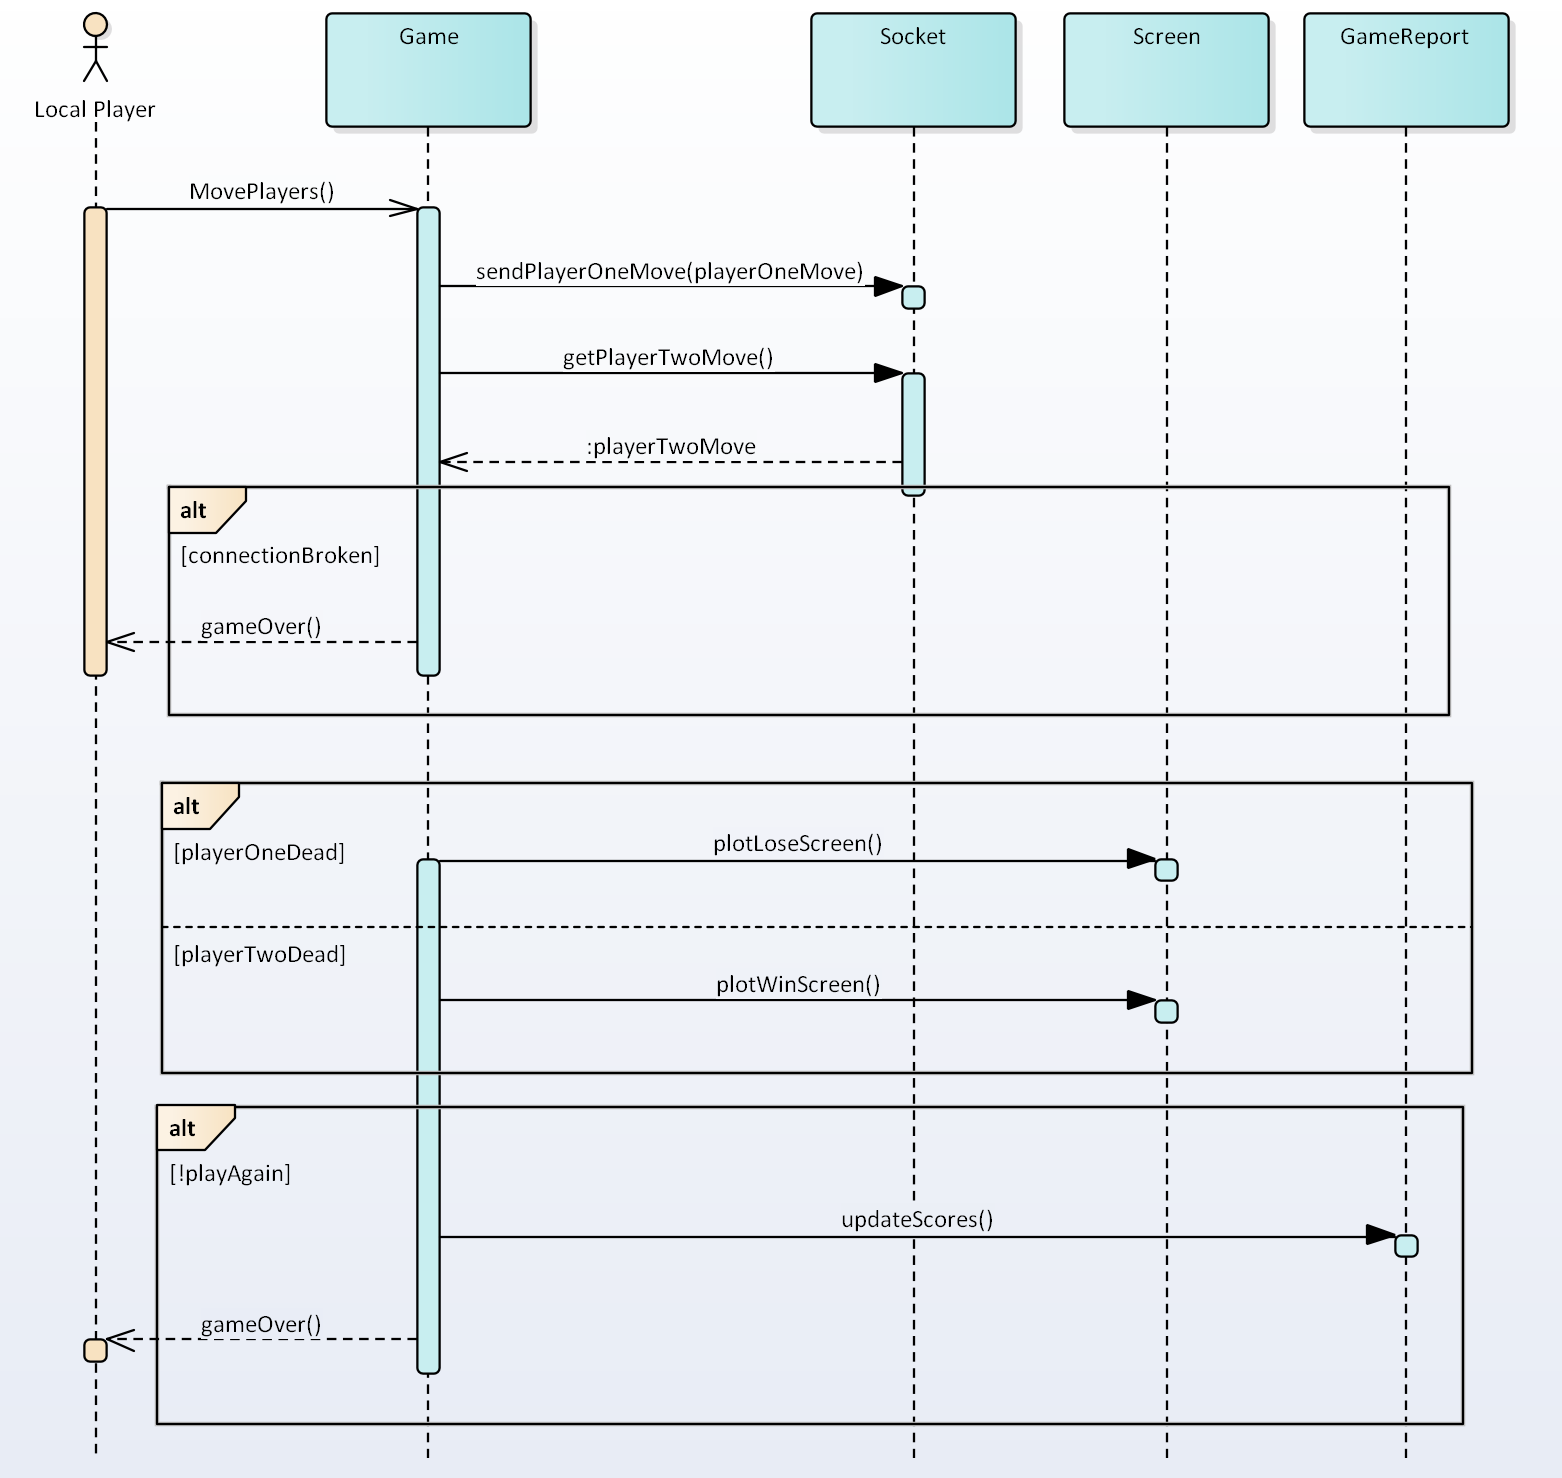
\includegraphics[scale=1]{Sequence2}
	
	\subsection{Sequence Diagram 3 : Play Again}
	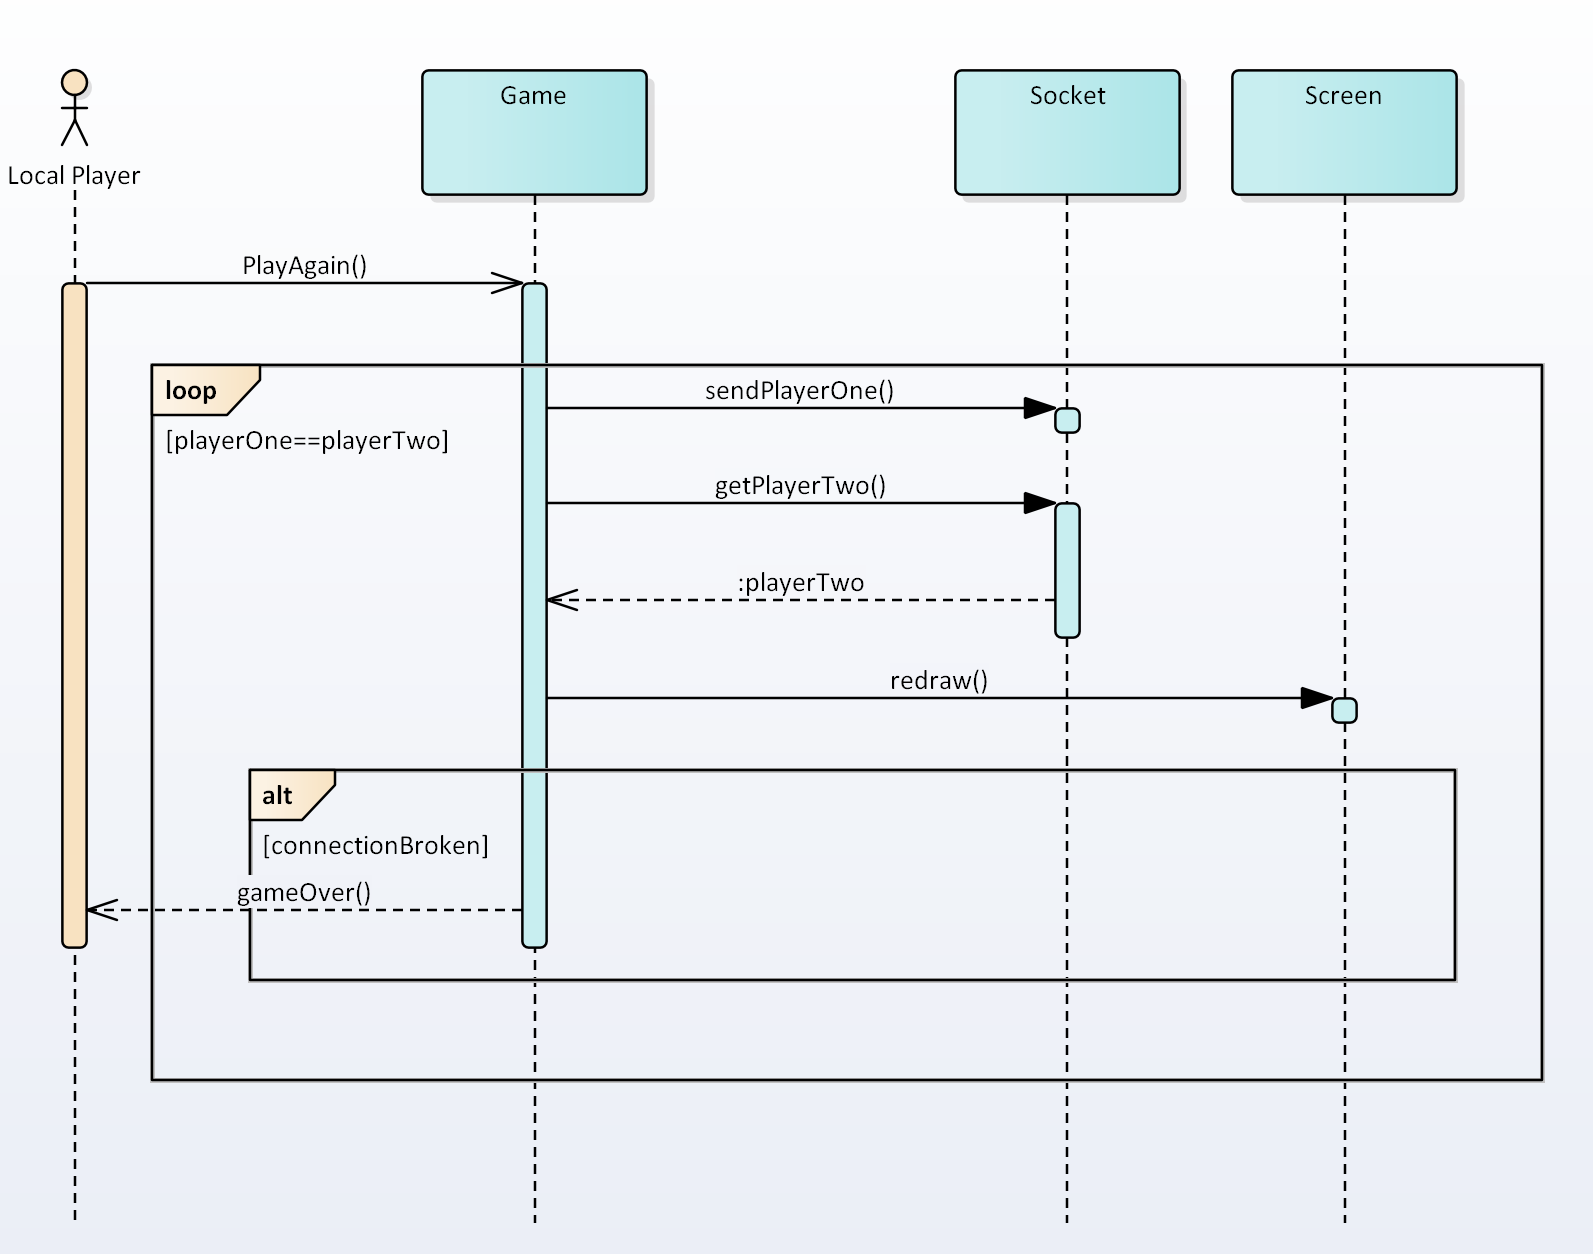
\includegraphics[scale=1]{Sequence3}
	
	\section{Design model}
	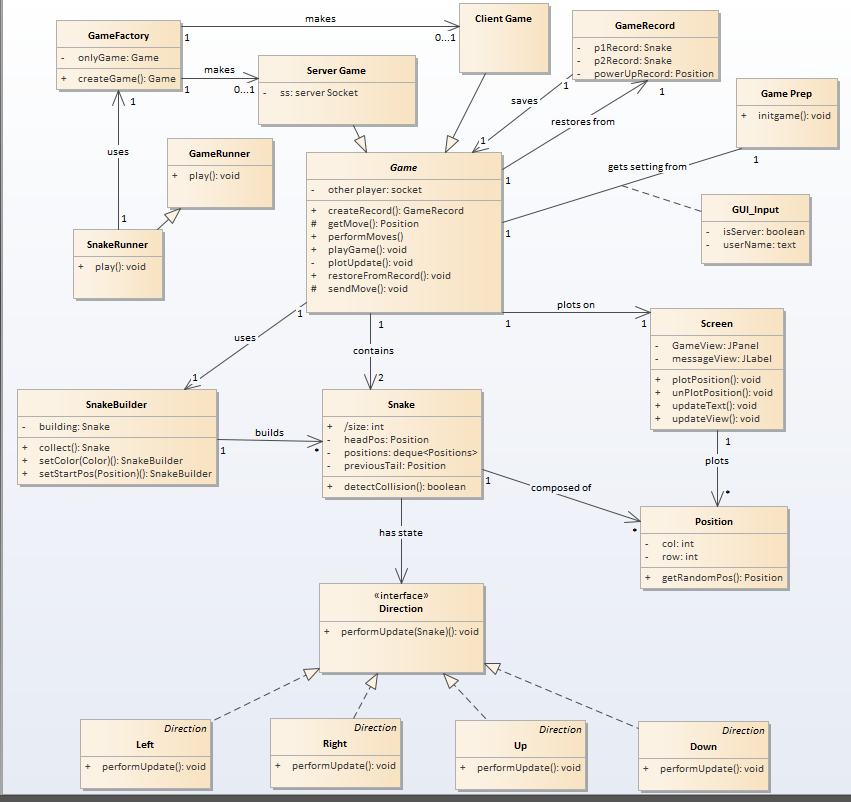
\includegraphics[scale=.75]{DesignModel_better}
	
	\section{GRASP}
		\begin{enumerate}
			\item \textbf{High Cohesion:}\\
			For high cohesion we focused on making sure that each class had one specific responsibility. For example the Game will handle all of the game logic, while the Screen is responsible for all display.
			\item \textbf{Pure Fabrication:}\\
			An example of pure fabrication in our project is the GameRecord class. It was introduced so that the Game state could be reverted.
			\item \textbf{Information Expert:}\\
			We delegated the creation of objects to the classes who know the required information. For example, the Wrapper is created by the Screen since the Screen knows what the width and height of the Wrapper need to be. Also, the only class that creates Snakes is the Game object.
			\item \textbf{Polymorphism:}\\
			The Game uses polymorphism when calculating the position that a Snake will move to. It is also used in Game so that the Game can properly act as either a server or a client.
		\end{enumerate}
	
	\section{Design Patterns}
		\begin{enumerate}
			\item \textbf{Singleton:}\\
				Singleton was the most used design pattern in this project. Many of the objects used lent themselves to only letting one instance exist at any
				time. The game screen and the game itself were both singletons.
			\item \textbf{Factory method:}
				Factory method was used to remove the need to use new to create instances of a Snake. The Cell method also had a getRandom method that functioned much like a factory.
			\item \textbf{Abstract Factory:}\\
				Abstract factory was used to create instances of a Game Object. Because there were multiple subtypes of the Game Object the abstract factory made it simpler to create an instance. Also the abstract factory allowed only one instance of any of game's subtypes to exist.
			\item \textbf{Builder:}\\
				A Builder is used to create instances of a Snake. Because the snake is a complex object builder lets the application customize them. It allows Snake location and color to be both be customized.
			\item \textbf{State:}\\
				State is used in the Screen to represent movement direction as determined by user keystrokes. It uses polymorphism to avoid using a switch statement in calculating the new snake position.
			\item \textbf{Command:}\\
				Command is used to represent the Game being executed. In this project there is only class that implements the GameRunner interface but it makes it so that new games you could easily be added to the project. The Main class runs a SnakeRunner which extends the abstract class GameRunner, and starts the SnakeGame;
			\item \textbf{Memento:}\\
				The memento design pattern is used when the players wish to restart the Game. It allows a version of the Game to be saved even though the Game is a singleton.
		\end{enumerate}
	\section{Stats}
	\subsection{Hours Spent per User}
	\textbf{Ian Laird:} ~~~~~25 hours\\
	\textbf{Andrew Walker:}~23 hours
	\subsection{Logical Lines from Each User}
	\textbf{Ian Laird:} ~~~~~ 574 lines\\
	\textbf{Andrew Walker:}~ 523 lines
\end{document}